\section{Introduction}

Using cooperative game theory to model bargaining outcomes has quite a few precedents in the economics literature.
This is, in part, motivated by the appealing properties of the resulting gain distributions and their tractability.
Furthermore, this practice also has solid theoretical justifications thanks to the long line of studies showing that various cooperative solution concepts are related to certain dynamic, non-cooperative bargaining games.\footnote{
    For example, \textcite{gul1989bargaining,winter1994demand,hart1996bargaining,inderst2003bargaining} propose various extensive-form bargaining games in which the equilibrium corresponds to players' Shapley values.
    For results specifically for games bargaining with one indispensable player, see \textcite{stole1996intra}.
}

The case of a small number of central players and a large number of fringe ones is particularly important in several settings.
Examples include intra-firm ownership structures \parencite{hart1990property}, wage bargaining \parencite{stole1996intra,stole1996organizational,levy1997individual}, collusion and mergers \parencite{segal2003collusion} and upstream-downstream supply chains \parencite{inderst2003bargaining,montez2007downstream}.
The study of multi-sided markets (or platforms) is also a good fit for this modeling approach, as platforms are often assumed to be indispensable for the various sides' interaction.\footnote{
    \textcite{huang2022shapley} is amongst the very few examples of using cooperative game theory in this setting.
}

I focus on how the central and fringe players split the total value that they can create.
By relying on a generalization of the Shapley value, namely, random order values\footnote{
    Similarly to the Shapley-value, random order values are also based on players' average marginal contributions to coalitions' values.
    Contrary to the Shapley value, this average can be taken with respect to any probability distribution.
}, this paper provides a general framework for modeling bargaining outcomes in this setting.
This also highlights the common themes between various results found in more applied papers.
I demonstrate that these values are described by tractable expressions and have geometric interpretations.
Just as importantly, I show that the outcomes align with one's intuitive expectations of bargaining power in such situations.

Apart from the general framework, this paper extends the results of the related literature in several ways.
Most importantly, I relax the usual assumption that there is only one indispensable player, and show how the results can be generalized when (1) there are multiple central players and (2) when the central player is not completely indispensable.
Further contributions include new results for the case of heterogeneous fringe players.
In particular, I provide results for weighted values in the case of heterogeneous fringe players, which is a novel contribution to the literature.
Furthermore, I highlight how the value of the fringe players can be expressed in terms of their marginal contributions (i.e. the partial derivatives of the production function).

I rely on an infinite-player (oceanic game) version of these models, where fringe players are represented as a continuum.
As is often the case in economics, this infinite-player approximation is more tractable than the finite-player model while retaining the latter's desirable features.
For example, the resulting profit shares depend on the production function in a similar way to how they do in the finite player case.
At the same time, they are continuous and differentiable functions of the size of the fringe.
The latter can be useful when embedding these results into more complex models.

The results presented in this paper can be used as a toolkit for embedding bargaining outcomes into more complex models.
To showcase the utility of this approach, I present a simple model of two-sided markets.
\applicationref{} provides a more full-fledged example of such an application, which relies on the results of the current paper to model bargaining outcomes in a market with a hybrid platform.

The present paper is closely related to two bodies of literature: a theoretical and an applied one.
Cooperative games with a finite number of atomic players and a continuum of non-atomic ones are called mixed or oceanic games \parencite{milnor1978values}, and have been studied in the cooperative game theory literature.
Generally, papers in this line of research focus on fundamental questions, such as the existence and uniqueness of the value \parencite{hart1973values}, and whether the various ways of defining it\footnote{
    One can characterize the value of the oceanic game directly, relying on a set of axioms (axiomatic approach). Alternatively, the value of an infinite-player game can also be defined as the limit of the value of a series of finite-player games (asymptotic approach).
} lead to the same result \parencite{fogelman1980asymptotic}.\footnote{
    \textcite{hart1973values} shows that in the case of mixed games, the usual axioms do not, in general, characterize a unique value.
    However, \textcite{fogelman1980asymptotic} demonstrates that, for a large subset of games, the asymptotic approach leads to one specific element from the set characterized by the axiomatic approach. 
}
My aim with this paper is both more general and more specific in certain aspects.
For one, I focus on the asymptotic approach and, within that, a specific way of approximating the game of interest.
This is motivated by the fact that I am not interested in the oceanic game per se but rather in its ability to approximate finite-player games.
Furthermore, I restrict my attention to a specific but economically significant subset of games: those with one (or a small number of) central player(s) and a continuum of fringe ones.
These two restrictions allow me to go beyond the Shapley value and obtain results for a more general set of solution concepts: random order values.
Additionally, instead of looking at general results, such as existence, I can provide and interpret explicit expressions for the values of the various players.

The other strand of research closely related to this paper belongs to the industrial organization literature, and, more specifically, to the literature on intermediation, multi-sided markets and vertical integration.
Despite their theoretical appeal and tractability, oceanic games saw remarkably little use in industrial organization and, more generally, applied economics.
Rare examples of such applications include \textcite{stole1996intra, stole1996organizational}\footnote{
    \textcite{stole1996intra} also provides microfoundations for using the Shapley value and the weighted value in a bargaining setting with one indispensable player.
} and \textcite{levy1997individual}, which use the Shapley value to model wage bargaining under a divisible labor assumption (continuum of workers).

The present paper contributes to this literature by providing a general framework for modeling bargaining outcomes in such settings, and highlighting some general properties of the various bargaining rules used in these papers.
The latter is achieved by relying on the concept of random order values, which includes the Shapley value and the weighted value as special cases.
The generalizations include relaxing the assumption on the indispensability of the central player, which is especially relevant in the context of competing platforms.
Additionally, I provide results on how the total value is distributed between the various players in the case of heterogeneous fringe when using weighted values.

Finally, the example application presented to demonstrate the usefulness of the proposed approach is based on the seminal work of \textcite{armstrong2006competition} on multi-sided markets.
Thus, despite the main results being presented in an abstract setting, this paper also has some minor contributions towards better understanding the functioning of platform economies.
In particular, it highlights that, in contrast to the unilateral price-setting case, under bargaining, entry fees for each side of the market do depend on the surplus realized on that side.\footnote{
    In the benchmark, unilateral price-setting model, the entry fee only depends on the externalities that the entrants impose and the elasticity of entry as a function of the entry fee.
}

The paper is organized as follows.
In \Cref{sec:one_sided}, I present the main results for the case of identical fringe players.
It includes generalizations that relax the assumption about the indispensability of the central player.
\Cref{sec:many_sided} then extends many of those results to the case of heterogeneous fringe players.
\Cref{sec:application} provides an example application of the results to a simple model of a two-sided market.
Finally, \Cref{sec:conclusions} concludes the paper.


\section{Identical fringe players}
\label{sec:one_sided}

In this section, I examine the case of identical fringe players.
I start with the case of one indispensable big player and then relax this assumption in \Cref{sec:extensions}.
Such a game can represent, for example, a (one-sided) platform and several potential entrants, where the entrants can only reach their prospective consumers through the platform, or a vertical supply chain with one upstream producer and many downstream sellers.
Let us start by defining the cooperative game that describes this situation.

Consider a game with two types of players: a central (or big) player $P$ and $n$ smaller players $A_i$, $1 \leq i \leq n$.
Formally, let us denote the set of all players as $N = \{P, A_1, \dots, A_n\}$.
Assume that (1) no coalition of players can achieve a positive value without the participation of $P$ and (2) players $A_i$ are identical to each other.
Let $n_T(S)$ denote the number of players of type $T \in \{P, A\}$ in coalition $S$.
Under these assumptions, the characteristic function of this game (the value that a coalition $S \subset N$ can achieve) is the following:
\begin{align*}
    v(S) = \begin{cases}
        0                              & \text{if } P \notin S \\
        f\left(\frac{n_A(S)}{n}\right) & \text{otherwise}.
    \end{cases}
\end{align*}
The function $f$ (henceforth the production function) then characterizes this game and determines the distribution of the value between the big player and the fringe.

Before delving into solution concepts, let us find conditions under which this game is monotone\footnote{
    Monotonicity requires that the value of any coalition is weakly higher than the value of any of its subsets.
} and superadditive\footnote{
    Superadditivity requires that the value of the union of two disjoint coalitions is weakly higher than the sum of their values.
}.
The latter is a key property of cooperative games, as it ensures that it always pays off to form the grand coalition (i.e., the coalition that includes all players).
Furthermore, in the context of bargaining, these properties provide theoretical support for using the Shapley value or the weighted value to represent bargaining outcomes, as many results that create a link between non-cooperative bargaining games and the values of cooperative games rely on these assumptions.\footnote{
    For example, the results in \textcite{gul1989bargaining} rely on superadditivity, while monotonicity suffices for \textcite[]{hart1996bargaining}.
}

As the following proposition shows, characterizing monotonicity and superadditivity is straightforward in this setting.
\begin{proposition}
    \label{prop:monotone}
    The game $(N, v)$ is monotone and superadditive if and only if $f$ is increasing and $f(0) \geq 0$.
\end{proposition}
The intuition behind this result is relatively straightforward.
As player $P$ is necessary to create any value, no two disjoint coalitions can both achieve a positive value.
Therefore, superadditivity is equivalent to monotonicity in this case.

In the following, let us assume that the assumptions required for monotonicity are always satisfied (i.e., $f$ is monotone increasing).\footnote{
    This assumption is not entirely innocuous.
    For example, having more small firms could, in theory, lead to stronger competition, decreasing total profits.
    However, it often holds in models with network effects \parencite{rochet2003platform} or with consumers having taste for variety \parencite{anderson2020aggregative}.
}
As a side note, it also ensures that the game is of bounded variation, and thus the main theorem in \textcite{fogelman1980asymptotic} applies.
Namely, the asymptotic and the axiomatic approach of characterizing the Shapley value of the game both lead to the same result\footnote{
    More precisely, the asymptotic value coincides with the axiomatic one derived using the uniform distribution.
    For a more detailed discussion, see \textcite{fogelman1980asymptotic}.
}.
This result observation can also be used to prove the main proposition about the Shapley value (\Cref{prop:one_sided}) instead of the direct proof provided in \Cref{sec:proofs}.

\subsection{Random order values}

Random order values are a class of cooperative solution concepts characterized by efficiency, monotonicity, linearity, and the null-player axiom \parencite{weber1988probabilistic}.
That is, they are a generalization of the Shapley value, with the axiom of symmetry being relaxed.
Another way to think about them is that they can be defined as the average marginal contribution of a player to all possible coalitions, where the average is taken according to some probability distribution over the players' permutations.

In this specific game, a random order value can be obtained in the following way.
First, take all permutations of the players, and assign a probability to each permutation.
Then, the corresponding random order value of player $P$ is the expected marginal contribution of $P$ to the value of the coalition preceding it, where the expectation is taken according to said probability distribution.

Random order values are of interest for several reasons.
First, they are a natural extension of the Shapley value and the weighted value.
Furthermore, they provide a convenient framework, of which all subsequent results (Shapley value, weighted value, multiple central players) are special cases.

For the remainder of the paper, let us use the following notation: $\varphi_P^n$ denotes the (depending on the section, Shapley, weighted or random order) value of player $P$ in the game with players $N = \{P, A_1, \dots, A_n\}$.
Then, formally,
\begin{align}
    \varphi_P^n = \frac{1}{(n+1)!} \sum_{R} \Pr(R) [ v(\precede_P^R \cup \{i\}) - v(\precede_P^R) ]  \label{eq:one_sided_general}
\end{align}
where $R$ is a permutation of all players, and $\precede_P^R$ denotes the set of players before $P$ in the permutation $R$. \footnote{
    For example, if $R = \{A_1, P, A_2\}$, then $\precede_P^R = \{A_1\}$.
}

Utilizing the fact that the value of any coalition is zero without $P$, and that -- conditional on player $P$ being in a coalition -- a coalition's value only depends on the number of fringe firms in it, the above expression can be simplified to the following:
\begin{align*}
    \varphi_P^n = \frac{1}{n+1} \sum_{k=0}^n \Pr(|\precede_P| = k) f(k/n),
\end{align*}
where $\Pr(|\precede_P| = k)$ is determined by the probability distribution over the permutations.

Now, let us look at the asymptotic limit of this expression as the number of fringe players goes to infinity.
The following proposition demonstrates the main idea of this paper: even as the number of fringe players goes to infinity, the value of the big player does not converge to the total worth of the grand coalition, $f(1)$.
Or, in other words, the fringe, even when its members are infinitesimally small, still retains some bargaining power.
As a consequence, the continuous fringe model can be considered a more tractable approximation of bargaining between a finite number of fringe players.

\begin{theorem}
    \label{prop:one_sided_general}
    Let $f$ be continuous on [0, 1]. Furthermore, let us denote the random variable $\frac{|\precede_P|}{n}$ as $X_n$. Assume that $X_n \xrightarrow[]{d} X$ with cdf $G(t)$ and (if exists) pdf $g(t)$.
    Then
    \begin{align*}
        \varphi_P^\infty = \lim_{n \to \infty} \varphi_P^n = \int_0^1 f(t) \dG(t) = \int_0^1 g(t) f(t) \dt,
    \end{align*}
    with the last equality holding if $X$ is a continuous random variable.
\end{theorem}

This result has an immediate interpretation in terms of marginal contributions.
Remember that player $P$ is indispensable for creating value.
Therefore, for any coalition of fringe players, the marginal contribution of player $P$ is the total value that the coalition can generate with $P$ included in it.
Player $P$'s average marginal contributionthen boils down to the expected value that a coalition can generate conditional on player $P$ being in it.

Now, let us turn to the value of the fringe.
The following corollary shows that the aggregated value of the fringe remains positive even in the limit.
In other words, even though the fringe players become smaller and more numerous, they do not lose all their bargaining power and still end up with a positive payoff.
\begin{corollary}
    \label{cor:fringe_value_general}
    The aggregated value of the fringe is
    \begin{align*}
        \varphi_A^\infty = f(1) - \int_0^1 f(t) \dG(t).
    \end{align*}
    Furthermore, if $f$ is differentiable on $[0, 1]$, then the value of the fringe can also be expressed as
    \begin{align*}
        \varphi_A^\infty = \int_0^1 G(t) f'(t) \dt.
    \end{align*}
\end{corollary}

This corollary also provides two ways of thinking about the value of the fringe.
First, because random order values are efficient, the fringe's share can be thought of as the leftover from the total value after subtracting the value of the big player.
Alternatively, as the second part of the corollary demonstrates, it is also related to the marginal contributions of the fringe agents.
This marginal contribution is the derivative of the production function (i.e., the effect of adding an infinitesimally small player to the coalition) multiplied by the probability of the central player appearing before a given fringe player (otherwise, the marginal contribution would be zero, as the central player is indispensable).
The second interpretation is particularly useful when thinking about the value of the fringe in a setting with heterogeneous fringe firms.

It also follows immediately from the previous proposition that (for a fixed total pie size $f(1)$) player $P$ gets a larger share when $f(t)$ is larger for every $t$.
That is, when only a relatively small fraction of the fringe is needed to create a large part of the total potential surplus, player $P$ can appropriate a larger share of the total value.
This result aligns with the intuition that player $P$ has a better bargaining position in this case than if only coalitions with most of the fringe firms on board could create considerable value.

In specific settings, this property of the production function can also be interpreted as the degree of complementarity or substitutability between the fringe players.
For example, imagine that the fringe consists of a set of firms producing one product each, and the central player is necessary for this product to be sold or created.\footnote{
    For example, the central player can be a platform that connects the fringe firms with consumers, or the provider of a key input.
}
When the fringe firms are substitutes, each additional one adds less value to the total pie.
Therefore, relatively few are needed to create most of the value, and the central player can appropriate a larger share.
Conversely, when the fringe firms are complements, the fringe firms are in a better bargaining position, and can obtain a larger share of the total value.


\subsection{Special cases}

This section discusses the two most important special cases of random order values: the Shapley value and the somewhat more general weighted value.
While most of these results are known in the literature, I include them here for two reasons: to build intuition for the more general case and to highlight the similarities to the model with heterogeneous fringe players.

\subsubsection{Shapley value}

Let us start with one of the most popular cooperative solution concepts, the Shapley value.
It can be characterized as the random order value that also satisfies the axiom of symmetry.
This axiom requires that if two players are identical in terms of the characteristic function, then they should have the same value.
Equivalently, it is the same as imposing that all permutations have an equal probability in \Cref{eq:one_sided_general}.

The following proposition and corollary derive the limit of the Shapley value for both types of players as the number of fringe players goes to infinity.

\begin{proposition}
    \label{prop:one_sided}
    Let $f$ be continuous on [0, 1]. Then
    \begin{align*}
        \varphi_P^\infty = \lim_{n \to \infty} \varphi_P^n = \int_0^1 f(t) \dt .
    \end{align*}
\end{proposition}

\begin{corollary}
    \label{cor:fringe_value}
    The aggregated Shapley value of the fringe is
    \begin{align*}
        \varphi_A^\infty = f(1) - \int_0^1 f(t) \dt.
    \end{align*}
    Furthermore, if $f$ is differentiable on $[0, 1]$, then the value of the fringe can also be expressed as
    \begin{align*}
        \varphi_A^\infty = \int_0^1 t f'(t) \dt.
    \end{align*}
\end{corollary}

Because the Shapley value is a special case of the random order values, these results are straightforward consequences of \Cref{prop:one_sided_general} and \Cref{cor:fringe_value_general}.
One only has to notice that each permutation having an equal probability implies that the number of firms coming before $P$ is uniformly distributed on $1, \dots, n$, and thus the share of firms before $P$ converges in distribution to the uniform distribution on $[0, 1]$.
Alternatively, a more direct proof is provided in \Cref{sec:proofs}, or a probabilistic justification can be found in \textcite{levy1997individual}.

The resulting Shapley values also have an instructive geometric interpretation shown on \Cref{fig:one_sided}.
Consider a rectangle with sides of length 1 and $f(1)$.
The grand coalition achieves the value $f(1)$, which is also the area of the rectangle.
The value of the big player is then $\int_0^1 f(t) \dt$, which is simply the part of the rectangle below the graph of $f$, while the fringe gets the rest.
Thus, the graph of $f$ partitions the area (total value) into what the big player and the fringe can obtain.

\begin{figure}
    \centering
    \begin{subfigure}[b]{0.45\textwidth}
        \centering
        \begin{tikzpicture}[scale=0.8]
            \begin{axis}[xmin=0, xmax=1, ymin=0, ymax=1, samples at={0, 0.02, ..., 0.98, 1},
                    xtick={0, 1}, ytick={0}, xlabel={$s$}]
                \addplot[name path=f, thick] {x^0.5};
                \node[anchor=north west] at (axis cs: .8, .8^0.5) {$f$};
                \path[name path=bottom] (axis cs:0,0) -- (axis cs:1,0);
                \path[name path=top] (axis cs:0,1) -- (axis cs:1,1);

                \addplot [fill=blue, fill opacity=0.05] fill between [of=f and bottom];
                \addplot [fill=red, fill opacity=0.05] fill between [of=f and top];

                \node[anchor=north west, align=left] at (axis cs: .05, .95) {Value of the \\ fringe ($\varphi_A^\infty$)};
                \node[anchor=south east, align=right] at (axis cs: .95, .05) {Value of the \\ big player ($\varphi_P^\infty$)};
            \end{axis}
        \end{tikzpicture}
        \caption{Fringe players have lower bargaining power}
        \label{fig:one_sided_substitute}
    \end{subfigure}
    \begin{subfigure}[b]{0.45\textwidth}
        \centering
        \begin{tikzpicture}[scale=0.8]
            \begin{axis}[xmin=0, xmax=1, ymin=0, ymax=1, samples at={0, 0.02, ..., 0.98, 1},
                    xtick={0, 1}, ytick={0}, xlabel={$s$}]
                \addplot[name path=f, thick] {x^1.5};
                \node[anchor=south east] at (axis cs: .8, .8^1.5) {$f$};
                \path[name path=bottom] (axis cs:0,0) -- (axis cs:1,0);
                \path[name path=top] (axis cs:0,1) -- (axis cs:1,1);

                \addplot [fill=blue, fill opacity=0.05] fill between [of=f and bottom];
                \addplot [fill=red, fill opacity=0.05] fill between [of=f and top];

                \node[anchor=north west, align=left] at (axis cs: .05, .95) {Value of the \\ fringe ($\varphi_A^\infty$)};
                \node[anchor=south east, align=right] at (axis cs: .95, .05) {Value of the \\ big player ($\varphi_P^\infty$)};
            \end{axis}
        \end{tikzpicture}
        \caption{Fringe players have higher bargaining power}
        \label{fig:one_sided_complement}
    \end{subfigure}
    \caption{Distribution of value between player $P$ (red) and the fringe (blue)}
    \label{fig:one_sided}
\end{figure}

Finally, the following corollary highlights that even though the individual share of each $A_i$ vanishes as their number goes to infinity, their total value remains positive.
\begin{corollary}
    \label{cor:fringe_value_2}
    $\varphi_P^\infty < f(1)$ and $\varphi_A^\infty > 0$ for any $f$ that is not constant.
\end{corollary}


\paragraph{Example: power function.}
\label{sec:power_function_example}

Let us illustrate the results of this section with a simple example.
Consider the case when $f(n) = n^\alpha$, for some $\alpha > 0$.
Assume that the bargaining occurs between player $P$ and a measure $\bar{n}$ of fringe players.
Thus, the value that the grand coalition can achieve is $\bar{n}^\alpha$.

\Cref{prop:one_sided} implies that the value of player $P$ in this case is
\begin{align*}
    \varphi_P^\infty(\bar{n}) = \int_0^1 (s \bar{n})^\alpha = \frac{1}{\alpha + 1} \bar{n}^\alpha,
\end{align*}
while the fringe gets the rest, i.e.,
\begin{align*}
    \varphi_A^\infty(\bar{n}) = \bar{n}^\alpha - \frac{1}{\alpha + 1} \bar{n}^\alpha = \frac{\alpha}{\alpha + 1} \bar{n}^\alpha.
\end{align*}

In other words, regardless of the value of $\bar{n}$, the two types of players share the total value in the same proportion.
This proportion depends on the parameter $\alpha$ (\Cref{fig:power_function_example}), which can be interpreted as the degree of substitutability between the fringe players.
More specifically, the higher $\alpha$ is, the more complementary the fringe players are to each other and the larger the share they obtain.
In the limit, when $\alpha \to \infty$, the fringe obtains all the value, as essentially all players become indispensable and share the total value equally.
On the other hand, when $\alpha \to 0$, the big player can appropriate all of the value.

\begin{figure}
    \centering
    \begin{tikzpicture}[scale=0.8]
        \begin{axis}[xmin=0, xmax=5, ymin=0, ymax=1, samples at={0, 0.05, ..., 4.95, 5},
                xtick={0, 1, 2, 3, 4, 5}, ytick={0, 1},
                xlabel={Complementarity between fringe players ($\alpha$)}, ylabel={Share of the fringe}]
            \addplot[name path=f, thick] {x / (1 + x)};
            \node[anchor=north west] at (axis cs: 3, 3/4) {$\frac{\varphi_A^\infty(\bar{n})}{f(\bar{n})}$};
            \path[name path=bottom] (axis cs:0,0) -- (axis cs:1,0);
            \path[name path=top] (axis cs:0,1) -- (axis cs:1,1);
        \end{axis}
    \end{tikzpicture}
    \caption{Example: share of the fringe as a function of $\alpha$ (degree of complementarity between fringe players)}
    \label{fig:power_function_example}
\end{figure}


\subsubsection{Weighted values}
\label{sec:weighted_one_sided}

The other important special case of random order values is the weighted value \parencite{shapley1953additive}.
It relaxes the symmetry axiom of the Shapley value and allows players to have different levels of innate bargaining power.
On the other hand, weighted values still have more structure than random order values, as they are characterized by a weight system that is more restrictive than assigning arbitrary probabilities to each permutation of players.
These weights determine how a coalition's value is distributed amongst its members when they are all equally important to the coalition.
Then, relying on the linearity of the value, this can be extended to the case when the players are not equally important.

The weights can be thought of as a measure of some innate bargaining power, which is not reflected in the production function.\footnote{
    However, this interpretation is not always appropriate.
    As \textcite{owen1968communications} demonstrates, there are games where the weighted value is not monotone increasing in a player's weight.
}
Further support for this interpretation in certain games can be found in \textcite{hart1996bargaining}, demonstrating that weights in a certain alternating offer bargaining game are related to the probability of each player making the offer.\footnote{
    For example, only one player having a positive weight corresponds to that player making take it or leave it offers.
}
Additionally, \textcite{stole1996intra} provides alternative microfoundations for the weighted value in the case of one indispensable and a continuum of fringe players.

For the purposes of the current players, it is sufficient to deal with the case of simple weights\footnote{
    In general, weighted values allow for more complex weight systems, with each player having a vector of weights applied in a lexicographic manner.
}
as I assume that there is at most one player with zero weight.
For the main result in this section, I make use of the following characterization of the weighted values: \textcite{kalai1987weighted} demonstrated that weighted values can be calculated by weighting the permutations by the probabilities arising from the following sequential ordering procedure.
Start with the set of all players.
Let the probability of player $i$ being the last amongst the set of remaining players $R$ be $\lambda_i / \sum_{j \in R} \lambda_j$.
Continue until all players are exhausted.
This yields a well-defined probability for each permutation of players.
The weighted value is then the same as the random order value with this probability distribution over the permutations.

Now, let us derive the weighted value and its limit for the big player and the fringe in this specific game.
I start by proving a lemma that characterizes the distribution of the number of players before $P$ in the limit.
Then, I use it to derive the weighted values of the players.

Consider the game described in the previous section, and let the weights of players of type $A$ and $P$ be 1 and $\lambda$, respectively.
Let $X_n$ be a random variable representing the number of players before $P$ when players are ordered according to the previously described procedure.
Then, the probability of player $P$ having at most $k$ players of type $A$ before themselves is simply
\begin{align}
    \label{eq:entry_distr_discrete}
    \Pr(X_n \leq k) = \prod_{j=k+1}^n \frac{j}{j + \lambda}.
\end{align}
The following lemma establishes the continuous analogue of this statement.
\begin{lemma}
    \label{lem:entry_distr}
    As $n \to \infty$, $X_n \xrightarrow[]{d} X$ with the cdf $G_X(t) = \lambda^t$.
    Consequently, the corresponding probability density function is $g(t) = \lambda t^{\lambda - 1}$.
\end{lemma}

With this in hand, deriving the weighted value of both types of players is straightforward.
Having \Cref{eq:entry_distr_discrete} and \Cref{lem:entry_distr} allows us to invoke \Cref{prop:one_sided_general} to obtain the following proposition.\footnote{
    \textcite{stole1996intra} also derive essentially the same expression for the equilibrium outcome of their bargaining game with unequal profit distribution and assert that it is equal to the weighted value.
}

\begin{proposition}
    \label{prop:one_sided_weighted}
    Let $f(t)$ be continuous on $[0, 1]$. Then
    \begin{align*}
        \varphi_P(\lambda, \infty) = \int_0^1 g(t) f(t) \dt
    \end{align*}
    where $g(t) = \lambda t^{\lambda - 1}$.

    Furthermore,
    \begin{align*}
        \varphi_A(\lambda, \infty) &= 1 - \int_0^1 g(t) f(t) \dt \\
                                &= \int_0^1 G(t) f'(t) \dt,
    \end{align*}
    where $G(t) = t^\lambda$.
\end{proposition}

As before, the value of the big player can be expressed as an integral of the production function, while the value of the fringe can be expressed as an integral of the marginal contributions of the fringe players.
The only difference is that, as in the case of the general random order value, the integrands are weighted by a specific probability distribution.
Depending on the shape of this distribution, regions corresponding to different masses of fringe firms can be over or underweighted in this integral, leading to different values.
Contrary to \Cref{prop:one_sided_general}, the probability distribution has a specific functional form and is characterized by a single parameter, $\lambda$.
\Cref{fig:weigh_function} illustrates the weighting function for various values of $\lambda$.

\begin{figure}[ht]
    \centering
    \begin{subfigure}[b]{0.45\textwidth}
        \centering
        \begin{tikzpicture}[scale=0.8]
            \begin{axis}[xmin=0, xmax=1, ymin=0, ymax=3, samples at={0.02, 0.04, ..., 0.98, 1},
                xtick={0, 1}, ytick={0, 1, 2, 3}, axis lines=left, xlabel={$t$}, legend pos=south east]
                \addplot[thick] {0.5 * x ^ (-0.5)};
                \addplot[thick, dashed] {1};
                \addplot[thick, dotted] {1.5 * x ^ (0.5)};
            \end{axis}
        \end{tikzpicture}
        \caption{$g(t)$}
    \end{subfigure}
    \begin{subfigure}[b]{0.45\textwidth}
        \centering
        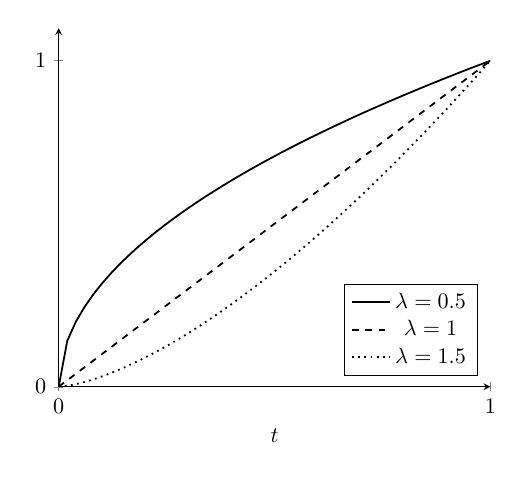
\begin{tikzpicture}[scale=0.8]
            \begin{axis}[xmin=0, xmax=1, ymin=0, ymax=1.1, samples at={0, 0.02, ..., 0.98, 1},
                xtick={0, 1}, ytick={0, 1}, axis lines=left, xlabel={$t$}, legend pos=south east]
                \addplot[thick] {x ^ (0.5)};
                \addplot[thick, dashed] {x};
                \addplot[thick, dotted] {x ^ (1.5)};
                \legend{$\lambda = 0.5$, $\lambda = 1$, $\lambda = 1.5$}
            \end{axis}
        \end{tikzpicture}
        \caption{$G(t)$}
    \end{subfigure}
    \caption{Illustration of the weighting function for various values of $\lambda$ in the weighted Shapley value.}
    \label{fig:weigh_function}
\end{figure}

Now, let us examine how these weights impact the shares of the various players.
It turns out that a higher weight corresponds to a higher value in this game.\footnote{
    This would not necessarily have to be the case, as demonstrated by \textcite{owen1968communications}.
},
supporting their interpretation as some kind of innate bargaining power.
\begin{corollary}
    \label{cor:platform_value_weighted}
    $\varphi_P(\lambda, \infty)$ is increasing in $\lambda$ unless $f$ is constant.
\end{corollary}

Furthermore, the following corollary shows that the limit of the weighted value of $P$, as their weight goes to zero (infinity), is precisely the payoff $P$ that they would achieve if they were making (facing) take-it-or-leave-it offers.
\begin{corollary}
    \label{cor:paltform_value_weighted_2}
    If the weight of player $P$ goes to infinity (zero), their weighted Shapley value converges to $f(1)$ ($f(0)$).
\end{corollary}
This set of results highlights that utilizing (weighted) Shapley values to model bargaining outcomes provides an intermediate solution between inscribing all the bargaining power to one type of player and, thus, ait is a generalization of take-it-or-leave-it offers, with the distribution of bargaining power being adjustable by a single parameter.


\subsection{Non-indispensable big player(s)}
\label{sec:extensions}

This section relaxes the assumption that the central player is indispensable.
I demonstrate two ways in which the model can be extended to include non-indispensable big players while retaining the essential structure and the tractability of the results.
In the first case, there is a finite number of big players who are perfect substitutes for each other.
In the second case, there is a single big player, but the fringe is able to generate some value on its own.
In both cases, the player's shares are still random order values\footnote{
    The case of multiple big players is equivalent to that of a single big player with the same production function but a different probability distribution over the permutations.
    Conversely, in the setting when the fringe can generate some value on its own, the production function changes, but the probability distribution is the same.
}, and thus, many of the earlier results apply.

\subsubsection{Multiple central players}

Imagine that, instead of just one, there are $m$ players of type $P$, and they are perfect substitutes for each other.
That is, any coalition still needs at least one of them to create any value, but it does not matter which and how many of them are present.\footnote{
    The relaxation of this assumption, while conceptually straightforward, is more complex to analyze.
    Instead of having to deal with the minimum of $m$ independent random variables, one needs to consider all order statistics.
}
Formally, the value function for coalition $S$ becomes the following:
\begin{align*}
    v(S) = \begin{cases}
        0                              & \text{if } n_P(S) = 0 \\
        f\left(\frac{n_A(S)}{n}\right) & \text{otherwise}.
    \end{cases}
\end{align*}

Let us start by establishing monotonicity for this version of the model, too.
\begin{proposition}
    The game is monotone if $f$ is increasing and $f(0) \geq 0$.
\end{proposition}
On the other hand, superadditivity is more complex in this case than before.
For example, when $f$ is concave, then $m$ coalitions with one platform each and the fringe divided equally amongst them achieve a higher total payoff than the grand coalition.
Therefore, the results of this section are most applicable to settings when multiple coalitions cannot be formed simultaneously.
For example, \textcite{hart1996bargaining} proposes that it might be due to a single, indivisible, non-replicable resource or technology (not captured in the value function) necessary to produce any value.

For simplicity, let us restrict our attention to probability distributions over the permutations which are symmetric with respect to the big players.
That is, the probability of having $k_F$ fringe players and $k_P$ big players before player $P_j$ is the same for all $i$.\footnote{
 This assumption can easily be relaxed, but it would complicate the results without adding much insight.
}
As before, I assume that, as the number of fringe players goes to infinity, the distribution of the number of fringe players before player $P_j$ converges to a continuous distribution.

Let us first establish the sum of the shares of all big players.
Then, the value of individual big players can be obtained by relying on the assumption of symmetry.
The following proposition provides an expression for the limit of this total value.
\begin{theorem}
    \label{prop:multiple_platforms_total}
    Let $f$ be continuous on [0, 1].
    Let us denote the number of fringe players in any coalition $S$ as $n_A(S)$.
    Furthermore, let us denote the random variable $\frac{n_A(\precede_{P_j})}{n}$ as $X_n^j$.
    Assume that $X_n^j$ and $X_n^k$ are independent for all $j \neq k$.
    Furthermore, suppose that $X_n^j \xrightarrow[]{d} X^j$ with cdf $G(t)$ and (if exists) pdf $g(t)$ for every $j = 1, \dots, m$.

    Let $H(t) = 1 - [1 - G(t)]^m$, i.e., the cdf of the minimum of the $m$ independent random variables distributed according to $G$.
    Then
    \begin{align*}
        \varphi_P^\infty = \lim_{n \to \infty} \sum_{j=1}^m \varphi_{P_j}^n = \int_0^1 f(t) \dH(t) = \int_0^1 h(t) f(t) \dt,
    \end{align*}
    with the last equality holding if $X$ is a continuous random variable.
\end{theorem}

Notably, value in the case of multiple, substitutable big players can reformulated as a random order value with a single big player.
The probability distribution for the corresponding random order value has a specific form, and depends on the number of big players.
Consequently, all the results from the previous section also apply to this case.

As with proposition \ref{prop:one_sided}, this result also has a probabilistic interpretation.
Let the location of the $m$ atoms be $t_1, \dots, t_m$, distributed independently and uniformly on the unit interval.
The expected marginal contribution of $t_i$ is only positive whenever it is the first amongst the central players.
Therefore, the total value of the big players is the random order value, with the corresponding probability distribution being the minimum of $m$ independent random variables describing the number of fringe players before each big player.

Due to the symmetry of the big players in terms of the permutation probabilities, the value of each individual big player is the same.
\begin{corollary}
    \label{prop:multiple_platforms_individual}
    The limit of the value (as $n \to \infty$) of each player of type $P$ is
    \begin{align*}
        \varphi_{P_i}^{\infty, m} = \frac{1}{m} \varphi_P^\infty = \int_0^1 \frac{h(t)}{m} f(t) \dt
    \end{align*}
    where $H(t) = 1 - [1 - G(t)]^m$, and $h(t) = H'(t)$ whenever $G$ is differentiable.
\end{corollary}
Furthermore, the value of the fringe has a similar, marginal contribution-based interpretation as in the case of a single big player.
\begin{corollary}
    \label{cor:multiple_platforms}
    The per-unit value of the fringe is
    \begin{align*}
        \varphi_A^{\infty, m} = 1 - \int_0^1 f(t) \dH(t) = \int_0^1 H(t) f'(t) \dt,
    \end{align*}
    where $H(t) = 1 - [1 - G(t)]^m$.
\end{corollary}

Finally, let us look at how the value of the big players and the fringe changes as a function of the number of the big players.
Proposition \Cref{cor:multiple_platforms_2} again confirms our intuition: more players means that they become more substitutable, and thus their bargaining power decreases.
This not only means that the value of each individual big player decreases but also that the sum of their values is reduced.
\begin{corollary}
    \label{cor:multiple_platforms_2}
    Let $\varphi_{P}^{\infty, m}$ denote the aggregated values of players of type $P$. $\varphi_{P}^{\infty, m}$ is decreasing in $m$ and $\varphi_{A}^{\infty, m}$ is increasing in $m$ unless $f$ is constant or $X$ is degenerate.
\end{corollary}

\paragraph{Example: Shapley value.}
I illustrate the effect of the number of central players on the weight function $h(t)$ by looking at the simplest of the random order values, the Shapley value.
As shown in \Cref{prop:one_sided}, the limit of the Shapley value in the case of a single big player is just $\int_0^1 f(t) \dt$.
Therefore, using the notation from \Cref{prop:one_sided_general}, $G(t) = t$.
Consequently, by \Cref{prop:multiple_platforms_total}, the sum of the shares of the big players corresponds to the random order value characterized by the cumulative distribution function
\begin{align} 
    H(t) = 1 - (1 - t)^m.  \label{eq:weight_function_shapley}
\end{align}
That is, the value of the sum of the big players' values is given by
\begin{align*}
    \varphi_P^{\infty, m} = \underbracket{m (1-t) ^ {m-1}}_{h(t)} f(t) \dt,
\end{align*}
while the value that each individual big player obtains is
\begin{align*}
    \varphi_{P_j}^{\infty, m} = \underbracket{(1-t) ^ {m-1}}_{h_j(t)} f(t) \dt.
\end{align*}

\Cref{fig:multiple_platforms,fig:multiple_platforms_total} illustrate how $h_t$ and $h_j(t)$ depend on the number of central players, $m$.
In particular, it is apparent that a $H(t)$ with lower $m$ first order stochastically dominates one with a higher number of players of type $P$.
This is the underlying reason for the big players' share decreasing in their number, i.e., \Cref{cor:multiple_platforms_2}.

\begin{figure}[ht]
    \centering
    \begin{subfigure}[b]{0.45\textwidth}
        \centering
        \begin{tikzpicture}[scale=0.8]
            \begin{axis}[xmin=0, xmax=1, ymin=0, ymax=1.1, samples at={0, 0.02, 0.04, ..., 0.98, 1},
                xtick={0, 1}, ytick={0, 1}, axis lines=left, xlabel={$t$}, legend pos=north west]
                \addplot[thick] {1};
                \addplot[thick, dashed] {1-x};
                \addplot[thick, dotted] {(1-x)^2};
            \end{axis}
        \end{tikzpicture}
        \caption{$h_i(t)$}
    \end{subfigure}
    \begin{subfigure}[b]{0.45\textwidth}
        \centering
        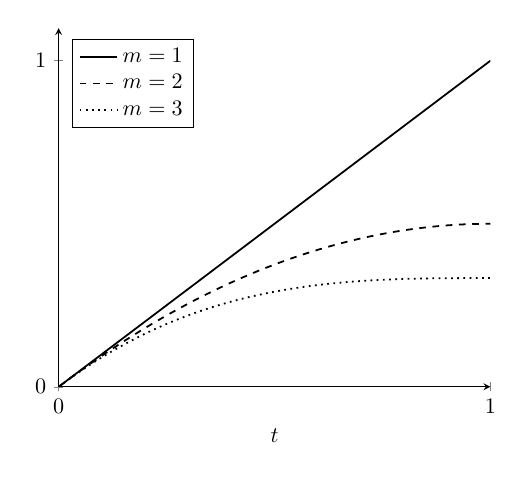
\begin{tikzpicture}[scale=0.8]
            \begin{axis}[xmin=0, xmax=1, ymin=0, ymax=1.1, samples at={0, 0.02, ..., 0.98, 1},
                xtick={0, 1}, ytick={0, 1}, axis lines=left, xlabel={$t$}, legend pos=north west]
                \addplot[thick] {x};
                \addplot[thick, dashed] {x - x^2/2};
                \addplot[thick, dotted] {x - x^2 + x^3/3};
                \legend{$m = 1$, $m = 2$, $m = 3$}
            \end{axis}
        \end{tikzpicture}
        \caption{$\int_0^t h_i(s) \ds$}
    \end{subfigure}
    \caption{Illustration of the weighting function for various values of $m$ in the multiple big player case -- individual big players.}
    \label{fig:multiple_platforms}
\end{figure}

\begin{figure}[ht]
    \centering
    \begin{subfigure}[b]{0.45\textwidth}
        \centering
        \begin{tikzpicture}[scale=0.8]
            \begin{axis}[xmin=0, xmax=1, ymin=0, ymax=3.1, samples at={0, 0.02, 0.04, ..., 0.98, 1},
                xtick={0, 1}, ytick={0, 1, 2, 3}, axis lines=left, xlabel={$t$}, legend pos=north west]
                \addplot[thick] {1};
                \addplot[thick, dashed] {2 * (1-x)};
                \addplot[thick, dotted] {3 * ((1-x)^2)};
            \end{axis}
        \end{tikzpicture}
        \caption{$h(t)$}
    \end{subfigure}
    \begin{subfigure}[b]{0.45\textwidth}
        \centering
        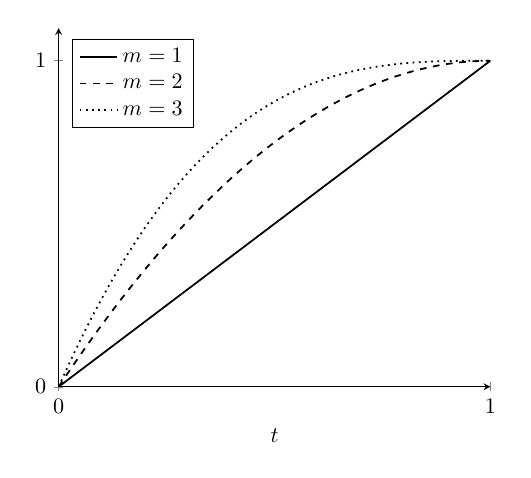
\begin{tikzpicture}[scale=0.8]
            \begin{axis}[xmin=0, xmax=1, ymin=0, ymax=1.1, samples at={0, 0.02, ..., 0.98, 1},
                xtick={0, 1}, ytick={0, 1}, axis lines=left, xlabel={$t$}, legend pos=north west]
                \addplot[thick] {x};
                \addplot[thick, dashed] {2 * (x - x^2/2)};
                \addplot[thick, dotted] {3 * (x - x^2 + x^3/3)};
                \legend{$m = 1$, $m = 2$, $m = 3$}
            \end{axis}
        \end{tikzpicture}
        \caption{$H(t) = \int_0^t h(s) \ds$}
    \end{subfigure}
    \caption{Illustration of the weighting function for various values of $m$ in the multiple big player case -- total of big players.}
    \label{fig:multiple_platforms_total}
\end{figure}


\subsubsection{Small players can generate some value on their own}

Another way of relaxing the central player's indispensability is to assume that the fringe players can generate some value on their own.
Suppose the big player still provides some value to any coalition, but a coalition of fringe players can achieve a positive value even without it.
Formally, the value function is now the following:
\begin{align*}
    v(S) = \begin{cases}
        f_0\left(\frac{n_A(S)}{n}\right) & P \notin S \\
        f\left(\frac{n_A(S)}{n}\right)   & \text{otherwise}.
    \end{cases}
\end{align*}

As with multiple central players, monotonicity is straightforward to establish.
\begin{proposition}
    The game is monotone if $f$ is increasing and $f(t) \geq f_0(t) \geq 0 \forall t$.
\end{proposition}
Also similarly, conditions for superadditivity are not as simple.
Therefore, the simultaneous formation of multiple coalitions must be assumed away in this setting, too.

On the other hand, the random order values and their limits are very straightforward to characterize.
The value of the big player is still its average marginal contribution.
The only difference is that this marginal contribution (conditional on $s$ share of the fringe coming before $P$) is not $f(s)$, but instead $f(s) - f_0(s)$.
This is because the big player is not indispensable, as $s$ mass of fringe firms can achieve $f_0(s)$ without it.

\begin{theorem}
    \label{prop:one_sided_non_indispensable}
    Let $f$ be continuous on [0, 1]. Furthermore, let us denote the random variable $\frac{|\precede_P|}{n}$ as $X_n$. Assume that $X_n \xrightarrow[]{d} X$ with cdf $G_X(t)$ and (if exists) pdf $g(t)$.
    Then
    \begin{align*}
        \varphi_P^\infty = \lim_{n \to \infty} \varphi_P^n = \int_0^1 f(t) \dG(t) = \int_0^1 g(t) [f(t) - f_0(t)] \dt,
    \end{align*}
    with the last equality holding if $X$ is a continuous random variable.
\end{theorem}

The value of the fringe is also similar to the baseline case, except now fringe players have a non-zero marginal contribution  to coalitions not containing player $P$.
Therefore, there is an additional term in the integral corresponding to the marginal value of fringe players when $P$ is not present.

\begin{corollary}
    \label{cor:fringe_value_non_indispensable}
    The aggregated value of the fringe is
    \begin{align*}
        \varphi_A^\infty = f(1) - \int_0^1 f(t) - f_0(t) \dG(t).
    \end{align*}
    Furthermore, if $f$ and $f_0$ are differentiable on $[0, 1]$, then the value of the fringe can also be expressed as
    \begin{align*}
        \varphi_A^\infty = \int_0^1 G(t) f'(t) + (1 - G(t)) f'_0(t) \dt.
    \end{align*}
\end{corollary}

Clearly, the value of the big player is decreasing in $f_0$ (\Cref{fig:non_indispensable}).
Consequently, the value of the fringe is increasing in $f_0$, which is essentially its outside option.
This is a natural result, and again, it aligns with what one would expect from bargaining theory.
\begin{figure}
    \centering
    \begin{subfigure}[b]{0.45\textwidth}
        \centering
        \begin{tikzpicture}[scale=0.8]
            \begin{axis}[xmin=0, xmax=1, ymin=0, ymax=1, samples at={0, 0.02, ..., 0.98, 1},
                    xtick={0, 1}, ytick={0}, xlabel={$s$}]
                \addplot[name path=f, thick] {x^0.5};
                \addplot[name path=f0, thick] {0.3 * x^0.5};
                \node[anchor=north west] at (axis cs: .8, .8^0.5) {$f$};
                \node[anchor=south west] at (axis cs: .8, .3*.8^0.5) {$f_0$};
                \path[name path=bottom] (axis cs:0,0) -- (axis cs:1,0);
                \path[name path=top] (axis cs:0,1) -- (axis cs:1,1);

                \addplot [fill=blue, fill opacity=0.05] fill between [of=f and f0];
                \addplot [fill=red, fill opacity=0.05] fill between [of=f and top];
                \addplot [fill=red, fill opacity=0.05] fill between [of=f0 and bottom];

                \node[anchor=north west, align=left] at (axis cs: .05, .95) {$\varphi_A^\infty$};
                \node[anchor=south east, align=left] at (axis cs: .95, .05) {$\varphi_A^\infty$};
                \node[anchor=north west, align=right] at (axis cs: .5, .5) {$\varphi_P^\infty$};
            \end{axis}
        \end{tikzpicture}
        \caption{Fringe can achieve relatively little without $P$}
    \end{subfigure}
    \begin{subfigure}[b]{0.45\textwidth}
        \centering
        \begin{tikzpicture}[scale=0.8]
            \begin{axis}[xmin=0, xmax=1, ymin=0, ymax=1, samples at={0, 0.02, ..., 0.98, 1},
                    xtick={0, 1}, ytick={0}, xlabel={$s$}]
                \addplot[name path=f, thick] {x^0.5};
                \addplot[name path=f0, thick] {0.7 * x^0.5};
                \node[anchor=north west] at (axis cs: .8, .8^0.5) {$f$};
                \node[anchor=north west] at (axis cs: .8, .7*.8^0.5) {$f_0$};
                \path[name path=bottom] (axis cs:0,0) -- (axis cs:1,0);
                \path[name path=top] (axis cs:0,1) -- (axis cs:1,1);

                \addplot [fill=blue, fill opacity=0.05] fill between [of=f and f0];
                \addplot [fill=red, fill opacity=0.05] fill between [of=f and top];
                \addplot [fill=red, fill opacity=0.05] fill between [of=f0 and bottom];

                \node[anchor=north west, align=left] at (axis cs: .05, .95) {$\varphi_A^\infty$};
                \node[anchor=south east, align=left] at (axis cs: .95, .05) {$\varphi_A^\infty$};
                \node[anchor=north west, align=right] at (axis cs: .5, .7) {$\varphi_P^\infty$};
            \end{axis}
        \end{tikzpicture}
        \caption{Fringe can achieve relatively more without $P$}
    \end{subfigure}
    \caption{Distribution of value between player $P$ (blue) and the fringe (red)}
    \label{fig:non_indispensable}
\end{figure}


\section{Heterogeneous fringe}
\label{sec:many_sided}

Until now, we have only considered games with a single type of small player.
Now imagine that, in addition to player $P$, there are $L$ different varieties of players: $\{A^l_1, \dots, A^l_n\}$ where $1 \leq l \leq L$.
The idea is the same as before: I assume that $P$ is necessary for any coalition to have a positive value, and the small players are identical to each other \emph{within their types}.
The -- now multivariate-- function $ f$ captures the substitutability of the different types of small players.

Let us now turn to the formal definition of the setting.
For a finite number of fringe players, the game's coalitional form, $(N, v)$, is the following.
The set of players is $N = \{P, A^1_1, \dots, A^1_n, \dots, A^L_1, \dots, A^L_n\}$, which in total contains $nL + 1$ players.\footnote{
 In this formulation, we assume that the number of players of each type is the same.
 However, this is not as restrictive as it might seem.
 In the limit, each type of player will become infinitesimally small, and the exact number of players of each type does not matter.
}
The characteristic function is
\begin{align*}
    v(S) = \begin{cases}
        0                                                & \text{if } P \notin S \\
        f\left(\frac{n_{A^1}(S)}{n}, \dots, \frac{n_{A^L}(S)}{n}\right) & \text{otherwise},
    \end{cases}
\end{align*}
where $f$ is now a multivariate function from $[0, 1]^L$ to $\mathbb{R}$ and $n_{A^l}(S)$ denotes the number of players of type $A^l$ in coalition $S$.

A prominent interpretation of the two-sided version of this model would be a platform marketplace with a set of sellers and a set of buyers, where all three sides possess some amount of bargaining power.
However, player $P$ does not have to be in the ``middle'' of the transactions for this framework to be applicable.
For example, it also captures the situation of a single upstream producer, a large number of downstream firms, and a similarly large number of customers, as long as both the customers and the downstream firms can participate in the bargaining process.\footnote{
    A setting where these assumptions might be plausible is, for example, the new car market, which has a car producer, several independent dealerships, and customers who might engage in some form of negotiation.
}
Models with more than two types of fringe players can represent, for example, a platform with more than two sides (such as buyers, sellers, and a set of advertisers) or, following \textcite{stole1996intra}, bargaining between a firm and multiple types of input providers.

The subsequent discussion follows the structure of \Cref{sec:one_sided}.
I start by characterizing conditions for monotonicity and superadditivity to support the bargaining interpretation of the results and the formation of the grand coalition.
It turns out that the necessary and sufficient conditions for these properties are straightforward analogs of those from the one-sided case.
\begin{proposition}
    The game $(N, v)$ is monotone and superadditive if and only if $f$ is increasing in all of its arguments.
\end{proposition}
The intuition for this is the same as before: superadditivity is equivalent to monotonicity due to the fact that no coalition can have a positive value without $P$, and monotonicity boils down to $f$ being increasing in all of its arguments.

In the following subsections, I first examine random order values and then the two most important special cases: the Shapley value and the weighted value.
Many of the results are similar to the one-sided case, including the marginal contribution interpretation of the fringe's value and the geometric interpretation of the Shapley value.
Furthermore, even though the number of fringe players is a multi-dimensional object in this case, for the limit of the Shapley and weighted values, one only has to integrate over a one-dimensional manifold within the unit hypercube, making the results more tractable.

\subsection{Random order values}

I start with the most general case: the random order value.
Let us establish the analog of \Cref{prop:one_sided_general} for the case of heterogeneous fringe to obtain the limit of the value of the big player.
\begin{theorem}
    \label{prop:many_sided_general}
    Let $f$ be continuous on $[0, 1]^L$. Furthermore, let us denote the random vector of the proportions of the various types of fringe players before $P$ as $X_n$:
    \begin{align*}
        X_n = \left( \frac{n_{A_1}(\precede_P)}{n}, \dots, \frac{n_{A_L}(\precede_P)}{n} \right).
    \end{align*}
    Assume that $X_n \xrightarrow[]{d} X$ with cdf $G_X(t_1, \dots, t_L)$ and (if exists) pdf $g(t_1, \dots, t_L)$.
    Then
    \begin{align*}
        \varphi_P^\infty = \lim_{n \to \infty} \varphi_P^n &= \int_0^1 \dots \int_0^1 f(t_1, \dots, t_L) \dG(t_1, \dots t_L) \\
        &= \int_0^1\dots \int_0^1 g(t_1, \dots, t_n) f(t_1, \dots, t_L) \dt_1 \dots \dt_L,
    \end{align*}
    with the last equality holding if $X$ is a continuous random variable.
\end{theorem}
The proposition above is almost identical to \Cref{prop:one_sided_general}, with the only difference being that the integral is now over the $L$-dimensional unit hypercube due to $f$ being a function of $L$ variables.

While the above proposition is very general in terms of permutation probabilities, its tractability in practice is hampered by the fact that one has to integrate over the entire $L$-dimensional domain of $f$.
It would be much more convenient if one only had to be concerned with some smaller, one-dimensional manifold within this hypercube.
It turns out that this is indeed the case for a number of important cases (namely, the Shapley value and the weighted value).

The following lemma states a general result about this idea: it provides sufficient conditions under which the limit of the value of the big player can be expressed as an integral over a one-dimensional path, even though the value for any finite number of players depends on the whole domain of $f$.
Later on I show that it applies to both the Shapley value and the weighted value.
\begin{lemma}
    \label{lem:many_sided_manifold}
    Assume that $X_n \xrightarrow[]{d} X$ where $X$ is a degenerate distribution in the following sense: $\exists \, a_l: [0, 1] \to [0, 1], l = 1, \dots, L$, such that
    \begin{align*}
        X = (a_1(\xi), \dots, a_L(\xi)),
    \end{align*}
    where $\xi$ is a random variable on $[0, 1]$ with cdf $H(s)$.
    In words, the whole probability mass is concentrated on the manifold $(a_1(s), \dots a_L(s)), t \in [0, 1]$.
    Then
    \begin{align*}
        \varphi_P^\infty = \lim_{n \to \infty} \varphi_P^n &= \int_0^1 f(a_1(s), \dots a_L(s)) \mathrm{d}H(s).
    \end{align*}
    Furthermore, if $f$'s partial derivatives exist on $\{(a_1(t), \dots, a_L(t)) : t \in [0, 1]\}$ the value of fringe $l$ has the following limit:
    \begin{align*}
        \varphi_{A^l}^\infty = \lim_{n \to \infty} \varphi_{A^l}^n &= \int_0^1 H(s) a_l'(s) \partial_l f(a_1(s), \dots a_L(s)) \ds.
    \end{align*}
\end{lemma}

The lemma states that if the permutation probabilities are such that the number of fringe players before $P$ converges to a degenerate distribution, then one only has to be concerned with just a tiny part of the production function $f$.
Namely, we only need to know how the function behaves on the set $\{(a_1(t), \dots, a_L(t)) : t \in [0, 1]\} \subset [0, 1]^L$.\footnote{
    For the fringe players, we also need the partial derivatives.
    Therefore, technically, the behavior of $f$ on some arbitrarily small neighborhood of this set also matters.
}
This result essentially generalizes the diagonal formula from \textcite{aumann2015values} or \textcite{stole1996intra} to the case where permutation probabilities are not uniform.
The intuition, however, is the same law-of-large-numbers-type argument: if the number of fringe players is large, then it is very improbable that, after a random ordering, their proportion in some subset of players is very different from its (conditional) expected value.
The main difference is that, in this case, these conditional expectations are not necessarily linear but rather given by the $a_l$ functions.

In the remainder of this section, I show that the Shapley value and the weighted value satisfy the assumptions of the above lemma
Thus, the limit of those values can be expressed as an integral over a well-defined, one-dimensional path.\footnote{
    I do not extend the heterogeneous agent model to the case of non-indispensable big players.
    It would be conceptually straightforward to do so for cases when \Cref{lem:many_sided_manifold} applies, albeit more cumbersome.
}

\subsection{Special cases}
\subsubsection{Shapley value}

Now, let us turn our attention to the Shapley value.
As hinted at earlier, due to the uniformity of the permutation probabilities, we obtain a diagonal formula in this case.
\Cref{prop:many_sided_shapley} establishes this result formally.

\begin{proposition}
    \label{prop:many_sided_shapley}
    Let $f$ be continuous on $[0, 1]^L$.
    Then,
    \begin{align*}
        \varphi_P^\infty & = \int_0^1 f(t, \dots, t) \dt
    \end{align*}
    and
    \begin{align*}
        \varphi_{A^l}^\infty = \int_0^1 t \partial_l f(t, \dots, t) \dt.
    \end{align*}
\end{proposition}
That is, in the case of the Shapley value, one has to integrate over the diagonal of the unit hypercube to obtain the limit of the value of the big player.\footnote{
    \textcite{stole1996intra} also obtain this expression for the big player's value for the limiting case of their bargaining game.
    The proof of this proposition demonstrates a way to obtain it as a limit of the Shapley value of the finite games.
}
\Cref{fig:many_sided_shapley} illustrates this result in the case of two types of fringe players: the value of player $P$ is the integral of $f$ over the diagonal of the unit square.
Furthermore, this result also demonstrates how the rest of the value is divided amongst the fringe players.
Namely, those having higher marginal contributions along the diagonal get a larger share of the value.

\begin{figure}
    \centering
    \begin{tikzpicture}
        \begin{axis}[
            xlabel={$a_1$}, ylabel={$a_2$}, zlabel={$f(a_1,, a_2)$},
            domain=0:1, y domain=0:1,
            zmin=0, zmax=1,
            xtick={0, 1}, ytick={0, 1}, ztick={0, 1},
            zticklabels={0, {$f(1, 1)$}}, % use the literal expression as a label
            view={60}{30}
        ]
            % plot the function
            \addplot3[surf, shader=flat, draw=none, name path=f, fill opacity=0] {x*y};
            % highlight the diagonal
            \addplot3[black, name path=diagonal, very thick, domain=0:1, samples=100, samples y=0] ({x}, {x}, {0});
            \addplot3[black, name path=f_diagonal, very thick, domain=0:1, samples=100, samples y=0] ({x}, {x}, {x^2});
            \addplot[blue, fill opacity=0.5] fill between[of=diagonal and f_diagonal];
        \end{axis}
    \end{tikzpicture}
    \caption{Illustration of the Shapley value in the case of two types of fringe players. The blue area corresponds to the value of the platform (with a scaling factor of $\sqrt{2}$ to account for the length of the diagonal)}
    \label{fig:many_sided_shapley}
\end{figure}


\subsubsection{Weighted value}

The final part of this section is dedicated to the weighted value in the heterogeneous fringe case.
The set of players and the characteristic function are the same as in the previous section, but, as before, each player has a weight attached to them.
I assume that fringe players of the same type have identical weights.
That is, the weight system for the game is the following: player $P$ has weight $\lambda_P$, while players $A^l_i$ have weight $\lambda_l$.

I will show that, as with the non-weighted Shapley value, the limit of the weighted value can also be expressed as an integral over a one-dimensional path in the weighted case.
However, this path is no longer the diagonal of the unit hypercube but a function of the fringe players' weights.
This is because not all permutations have the same probability of occurring: those with players having higher weights ordered later are more likely to occur.

The following statement is the central theorem of this paper.
Many of the propositions with one indispensable player can be considered as special cases of it.
\begin{proposition}
    \label{prop:many_sided_weighted}
    Let $f$ be continuous on $[0, 1]^L$.
    Then,
    \begin{align*}
        \varphi_P^\infty & = \int_0^1 \lambda_P t^{\lambda_P - 1} f(t^{\lambda_1}, \dots, t^{\lambda_L}) \dt
    \end{align*}
    and
    \begin{align*}
        \varphi_{A^l}^\infty & = \int_0^1 t^{\lambda_P} \lambda_l t^{\lambda_l - 1} \partial_l f(t^{\lambda_1}, \dots, t^{\lambda_L}) \dt.
    \end{align*}
\end{proposition}
The intuition for this is the following.
A higher weight for a player means that it has a higher chance of being relatively late in a random permutation.
Therefore, conditional on $s$ proportion of the fringe coming before $P$, the various types' proportions do not reflect their population shares ($1/L$).
For any $s \in (0, 1)$, the proportion of fringe players with a higher weight is lower than their population share, while the proportion of fringe players with a lower weight is higher than their population share.

\Cref{fig:many_sided_weighted} illustrates this phenomenon in the case of two types of fringe players.
Players of type $A^2$ have a higher weight than those of type $A^1$, and thus, the path the integral is taken over contains more of the latter than the former.

Finally, player $P$'s probability of coming after $s$ proportion of the fringe is also not uniform but rather influenced by the relationship between its own and the fringe players' weights.\footnote{
    This is the same mechanism as in the case of the one-sided weighted value.
} 
Therefore, the integral is not taken with respect to the uniform distribution, but rather one resembling that in \Cref{prop:one_sided_weighted}.
Its effect is also the same: when the big player has a higher weight, its chances of being relatively late in the ordering are higher, and thus -- due to $f$ being monotone increasing -- its value is higher.
The following simple corollary formalizes this idea.

\begin{figure}
    \centering
    \begin{tikzpicture}
        \begin{axis}[
            xlabel={$a_1$}, ylabel={$a_2$}, zlabel={$f(a_1,, a_2)$},
            domain=0:1, y domain=0:1,
            zmin=0, zmax=1,
            xtick={0, 1}, ytick={0, 1}, ztick={0, 1},
            zticklabels={0, {$f(1, 1)$}}, % use the literal expression as a label
            view={60}{30}
        ]
            % plot the function
            \addplot3[surf, shader=flat, draw=none, name path=f, fill opacity=0] {x*y};
            % highlight the diagonal
            \addplot3[black, name path=diagonal, very thick, domain=0:1, samples=100, samples y=0] ({x}, {x^3}, {0});
            \addplot3[black, name path=f_diagonal, very thick, domain=0:1, samples=100, samples y=0] ({x}, {x^3}, {x^4});
            \addplot[blue, fill opacity=0.5] fill between[of=diagonal and f_diagonal];
        \end{axis}
    \end{tikzpicture}
    \caption{Illustration of the weighted value in the case of two types of fringe players. Players of type $A^2$ have a higher weight than those of type $A^1$, thus the integral is not taken over the diagonal. The blue area corresponds to the value of the platform (the area have to be scaled so that the length of the path integrated over is one)}
    \label{fig:many_sided_weighted}
\end{figure}

\begin{corollary}
    \label{cor:platform_value_multiple_sides_weighted}
    $\varphi_P^\infty$ is increasing in $\lambda_P$ unless $f$ is constant.
\end{corollary}
This result is analogous to \Cref{cor:platform_value_weighted} and demonstrates that a higher weight for player $P$ corresponds to a higher value in this game, as well.

\section{Example application}
\label{sec:application}

In this section, I apply the ideas from the previous sections to a simple model of two-sided platforms.
I follow the modeling approach of \textcite{armstrong2006competition}, focusing on the monopolist platform case.
The model presented in this section expands on the original in two main ways.
First, and most importantly, I add bargaining between the platform and the two sides.
That is, besides the welfare-maximizing and unilateral price-setting cases presented in \textcite{armstrong2006competition}, I also consider a case where the platform and the two sides bargain over the entry fees.
I assume that the outcomes of this bargaining process are described by the weighted value.
Second, instead of assuming that each player's utility is linear in the number of the other side's size, I allow for more general non-linear network effects. 
This extension lets me capture and vary the substitutability of the players on each side.

\subsection{Model}

Consider a two-sided market with a continuum of players on both sides, and a single platform connecting those two sides.
Furthermore, assume that the utility that a player on side $i$ derives from participating in this market is an increasing function\footnote{
    \textcite{armstrong2006competition} -- along with much of the early literature on two-sided markets \parencite[e.g.][]{rochet2003platform,hagiu2006pricing} -- assume that the utility of each player is linear in the number of players on the other side.
    Using a more general function allows for modeling different kinds of network effects.
} of the number of players on the other side ($n_j$), minus the entry fee charged by the platform ($p_i$):
\begin{align*}
    u_i = \alpha_i n_j ^ {\gamma_i} - p_i.
\end{align*}
In this formulation, $\alpha \geq 0$ and $\gamma > 0$ determine the strength and shape of the network effects, respectively.

Following \textcite{armstrong2006competition}, I also model player entry in a reduced form manner.
Assume that there is a continuum of potential entrants on both sides of the market.
The number of actual entrants depends on the utility they would derive from participating if they entered.
Let us denote this relationship as $\phi_i(u_i)$, where $\phi_i$ is a strictly increasing, differentiable function.\footnote{
    Such assumptions are usually justified by having idiosyncratic cost entry costs, the distribution of which determines the function $\phi$.
    For simplicity, I refrain from explicitly modeling this cost in the main text, but \Cref{sec:explicit_entry_costs} discusses how one can incorporate it into the model and how it impacts bargaining outcomes.
}
Then,
\begin{align*}
    n_i = \phi_i(u_i).
\end{align*}

Finally, let us assume that the platform can charge lump-sum entry fees to both sides.
These fees are allowed to be negative, in which case they can be interpreted as subsidies.
The platform's profit is the sum of entry fees minus the cost of serving the entrants ($F_i$ for each entrant):
\begin{align*}
    \pi(n_1, n_2) = n_1 p_1 + n_2 p_2 - F_1 n_1 - F_2 n_2.
\end{align*}

I consider two cases as to the determination of the entry fees, as well as a welfare-maximizing benchmark.
In the benchmark case, I derive the entry fees that maximize social welfare (i.e., the sum of the utilities of the two sides plus the platform's profit).
After that, I consider a model analogous to that in \textcite{armstrong2006competition}, where the platform can unilaterally commit to any entry fees.
Finally, I examine and contrast the case where the entry fees result from a bargaining process such that the resulting utilities and profits correspond to the players' (weighted) values.

\subsection{Welfare-maximizing entry fees}

Let us first consider what the entry fees would be if they were set to maximize social welfare.
Instead of approaching this problem directly, I rely on the following observation: if entry fees correspond to the externality that a player's entry imposes on others, then the resulting entry decisions are welfare-maximizing.

In this specific case, there are two externalities to consider: (1) it costs the platform $F_i$ to serve an additional player on side $i$, and (2) the entry of a player on side $i$ increases the utility on side $j$ due to the presence of network effects.
Welfare is maximized when the price reflects the balance of these two factors.
\begin{proposition}
    \label{prop:welfare_max_entry_fees}
    The welfare-maximizing entry fees for side $i$ are characterized by
    \begin{align}
        p_i^* = F_i - \alpha_j \gamma_j n_j n_i^{\gamma_j - 1}.  \label{eq:welfare_max_entry_fees}
    \end{align}
\end{proposition}

Similarly to \textcite{armstrong2006competition}, for any $\alpha_j > 0$, the welfare-maximizing entry fee $F_i$ is below the platform's cost of serving player $i$.
As a consequence, the platform makes negative profits.
Therefore, while this case is useful as a benchmark, it is not particularly realistic when the platform has a say in determining entry fees, or has the possibility to exit the market altogether.

As an immediate corollary to \Cref{prop:welfare_max_entry_fees}, utilities in this case are given by
\begin{align*}
    u_i^*(n_i, n_j) = \alpha_i n_j ^ {\gamma_i} + \alpha_j \gamma_j n_j n_i^{\gamma_j - 1} - F_i
\end{align*}
for each individual player on side $i$.
The total welfare on side $i$ is, in turn, given by
\begin{align}
    W_i^*(n_i, n_j) = \alpha_i n_i n_j ^ {\gamma_i} + \gamma_j \alpha_j n_j n_i^{\gamma_j} - n_i F_i.
\end{align}

That is, players on side $i$ obtain the total generated by themselves, plus $\gamma_j$ times the total utility generated by the other side, minus the cost of serving them.
The utility of side $i$ depends positively on both $\alpha_i$ (mechanically) and $\alpha_j$ (a stronger positive externality on the other players implies a lower entry fee and thus higher utility).
Furthermore, it is increasing in the number of entrants on the other side through two channels: (1) entrants on the other side generate utility for side $i$ through network effects, and (2) players on side $i$ are compensated for the positive externality they impose on each player on the other side.

The effects of $\gamma_j$ are somewhat more complex and are best understood through the dependence of the utility of side $i$ on $n_i$.
Total welfare on side $i$ is always increasing in $n_i$, but individual utilities do not have to be.
If $\gamma_j > 1$ (i.e., network effects are convex), then $u_i$ is indeed increasing in $n_i$, as the positive externality each player imposes on the other side is increasing in the number of entrants.
Conversely, when $\gamma_j < 1$, the positive externality of the whole side is still increasing in their number (therefore, $W_i$ is increasing in $n_i$), but the positive externality each individual player imposes is now a decreasing function of it (thus, $u_i$ is decreasing in $n_i$).

\subsection{Platform sets prices unilaterally}

Now, let us examine what happens when the platform can set the entry fees unilaterally.
First, let us rewrite the platform's profit as a function of utilities instead of number of entrants:
\begin{align*}
    \pi_P(u_1, u_2) = \phi_1(u_1) [\alpha_1 \phi_2(u_2) ^ {\gamma_1} - u_1 - F_1] + \phi_2(u_2) [\alpha_2 \phi_1(u_1) ^ {\gamma_2} - u_2 - F_2].
\end{align*}
If the platform can set entry fees unilaterally, then its problem can be viewed as choosing $u_1$ and $u_2$ to maximize this expression.
The following proposition characterizes the solution of this maximization problem.
\begin{proposition}
    \label{prop:unilateral_entry_fees}
    Assume that $\pi_P(u_1, u_2)$ is concave in $u_i$ and $u_2$.
    Then, the profit-maximizing entry fees for side $i$ are characterized by
    \begin{align}
        p_i^u &= F_i - \alpha_j \gamma_j n_j n_i^{\gamma_j - 1} + \frac{\phi_1(u_1)}{\phi'_1(u_1)}  \label{eq:unilateral_entry_fees} \\
              &= p_i^* + \frac{\phi_1(u_1)}{\phi'_1(u_1)}.  \nonumber
    \end{align}
\end{proposition}

As one would expect, profit-maximizing entry fees are higher than welfare-maximizing ones.
In addition to the comparative statics of the welfare-maximizing case, unilaterally chosen entry fees also depend on the elasticity of entry.
When this elasticity is low, the platform can set high entry fees, as the resulting reduction in the number of entrants is relatively minor.

For ease of comparison with the bargaining case, let us  also derive the individual utilities and total welfare on each side:
\begin{align*}
    u_i^u(n_1, n_2) &= \alpha_i n_j ^ {\gamma_i} + \alpha_j \gamma_j n_j n_i^{\gamma_j - 1} - F_i - \frac{\phi_1(u_i)}{\phi'_1(u_i)} \\
    W_i^u(n_1, n_2) &= \alpha_i n_i n_j ^ {\gamma_i} + \gamma_j \alpha_j n_j n_i^{\gamma_j} - n_i F_i - n_i^2 (\phi_i^{-1})'(n_i).
\end{align*}
As expected, equilibrium utilities are smaller than in the welfare-maximizing case.
Due to $\phi_i$ being increasing, the number of entrants is also lower.

\subsection{Bargaining}

Finally, let us consider the case when the platform and the entrants bargain over the value they generate.
Suppose that $n_1$ and $n_2$ players have decided to enter on sides $1$ and $2$, respectively.
Furthermore, assume that players' bargaining weights are $\lambda_1, \lambda_2$, and $\lambda_P$.

The characteristic function of the game takes a similar form to that in \Cref{sec:many_sided}.
If the platform is not a member of a coalition, then that coalition can generate no value.
Otherwise, the value of the coalition is the sum of the utilities of the two sides minus the cost of serving them:\footnote{
    Entry fees paid to the platform do not matter as they are within-coalition transfers, and thus do not affect the total value.
}
\begin{align*}
    w(n_1, n_2) = n_1 \alpha_1 n_2^{\gamma_1} + n_2 \alpha_2 n_1^{\gamma_2} - F_1 n_1 - F_2 n_2.
\end{align*}

The share received by each type of player can then be established using \Cref{prop:many_sided_weighted}.
\begin{proposition}
    \label{prop:bargaining_entry_fees}
    The weighted values of the various sides are
    \begin{alignat*}{4}
        \pi_P^b(n_1, n_2) &= \underbracket{\frac{\lambda_P}{\lambda_P + \lambda_1 + \lambda_2\gamma_1}}_{\coloneqq S_P^{b_1}} \alpha_1 n_1 n_2^{\gamma_1} &&+ \underbracket{\frac{\lambda_P}{\lambda_P + \lambda_2 + \lambda_1\gamma_2}}_{\coloneqq S_P^{b_2}} \alpha_2 n_2 n_1^{\gamma_2} &&- \underbracket{\frac{\lambda_P}{\lambda_P + \lambda_1}}_{\coloneqq S_P^{c_1}} n_1 F_1 &&- \underbracket{\frac{\lambda_P}{\lambda_P + \lambda_2}}_{\coloneqq S_P^{c_2}} n_2 F_2 \\
        W_1^b(n_1, n_2) &= \underbracket{\frac{\lambda_1}{\lambda_P + \lambda_1 + \lambda_2\gamma_1}}_{\coloneqq S_1^{b_1}} \alpha_1 n_1 n_2^{\gamma_1} &&+ \underbracket{\frac{\lambda_1 \gamma_2}{\lambda_P + \lambda_2 + \lambda_1\gamma_2}}_{\coloneqq S_1^{b_2}}  \alpha_2 n_2 n_1^{\gamma_2} &&- \underbracket{\frac{\lambda_1}{\lambda_P + \lambda_1}}_{\coloneqq S_1^{c_1}} n_1 F_1 && \\
        W_2^b(n_1, n_2) &= \underbracket{\frac{\lambda_2\gamma_1}{\lambda_P + \lambda_1 + \lambda_2\gamma_1}}_{\coloneqq S_2^{b_1}} \alpha_1 n_1 n_2^{\gamma_1} &&+ \underbracket{\frac{\lambda_2}{\lambda_P + \lambda_2 + \lambda_1\gamma_2}}_{\coloneqq S_2^{b_1}} \alpha_2 n_2 n_1^{\gamma_2} && &&- \underbracket{\frac{\lambda_2}{\lambda_P + \lambda_2}}_{\coloneqq S_2^{c_2}} n_2 F_2.
    \end{alignat*}
\end{proposition}

Total welfare $w(n_1, n_2)$ can be divided into four parts: utility generated by sides $1$ and $2$, and the costs of serving sides $1$ and $2$.
Each side's share of these parts is given by $S_i^{b_1}, S_i^{b_2}, S_i^{c_1}$ and $S_i^{c_2}$, respectively.
As it turns out, these shares only depend on the bargaining weights ($\lambda_P, \lambda_1, \lambda_2$) and the network effects ($\gamma_1, \gamma_2$), but not on the actual number of entrants.\footnote{
    This is due to the characteristic function being a polynomial of the number of entrants.
    Just like in \Cref{sec:power_function_example}, each constituent of the polynomial is divided in a constant proportion.
}
Furthermore, all of these shares are increasing in one's own bargaining weight and decreasing in the others' weights.
Finally, and perhaps most interestingly, the share of side $i$ from the value generated on side $j$ is also increasing in $\gamma_j$.
This means that if players on side $i$ are less substitutable (or, equivalently, more complementary) in terms of contributing to the utility of the other side, then they will receive a larger portion of the value generated there.

These expressions for welfare are remarkably similar in structure to those obtained in the welfare maximizing case.
The main difference is that each part (both costs and positive utilities) is reweighted, and either side only receives a fraction of it.
These similarities and differences are examined in more detail in \Cref{sec:application_comparison}.

To make comparisons easier, let us also derive implied entry fees and utilities.\footnote{
    If one wished to close the model, the number of entrants in equilibrium could be obtained by solving the system of equations $n_i = \phi_i(u_i(n_1, n_2)), n \in \{1, 2\}$, just like in the other cases.
}
The latter is simply average welfare, i.e.
\begin{align*}
    u_i^b(n_1, n_2) &= \frac{\lambda_i}{\lambda_P + \lambda_i + \lambda_j\gamma_i} \alpha_i n_j^{\gamma_i} + \frac{\lambda_i \gamma_j}{\lambda_P + \lambda_j + \lambda_i\gamma_j} \alpha_j n_j n_i^{\gamma_j - 1} - \frac{\lambda_i}{\lambda_P + \lambda_i} F_i.
\end{align*}
Implied entry fees, on the other hand, can be calculated from the equation $u_i = \alpha_i n_j^{\gamma_i} - p_i$, yielding
\begin{align}
    p_i^b(n_1, n_2) &= \frac{\lambda_i}{\lambda_P + \lambda_i} F_i - \frac{\lambda_i \gamma_j}{\lambda_P + \lambda_j + \lambda_i\gamma_j} \alpha_j n_j n_i^{\gamma_j - 1} + \frac{\lambda_P + \lambda_j\gamma_i}{\lambda_P + \lambda_i + \lambda_j\gamma_i} \alpha_i n_j^{\gamma_i}.  \label{eq:bargaining_entry_fees}
\end{align}

\subsection{Comparison}
\label{sec:application_comparison}

Let us now compare the outcomes of the three cases described in the previous sections.
To highlight the similarity to \textcite{armstrong2006competition}, I first consider the case of linear network effects.
Furthermore, for simplicity of exposition, I start by examining the non-weighted Shapley value before moving on to the weighted value.

Therefore, first assume that network effects are linear, i.e., $\gamma_i = 1$ for $i \in \{1, 2\}$ and that all players have equal weights ($\lambda_P = \lambda_1 = \lambda_2 = 1$).
From \Cref{eq:welfare_max_entry_fees,eq:unilateral_entry_fees,eq:bargaining_entry_fees}, the entry fees for side $i$ are
\begin{align*}
    p_i^* &= \underbracket{F_i}_{(1)} - \underbracket{\alpha_j n_j n_i}_{(2)}, \\
    p_i^u &= \underbracket{F_i}_{(1)} - \underbracket{\alpha_j n_j n_i}_{(2)} + \underbracket{n_i (\phi_i^{-1})'(n_i)}_{(3)} \\
    p_i^b &= \underbracket{\frac{1}{2} F_i}_{(1)} - \underbracket{\frac{1}{3} \alpha_j n_j n_i}_{(2)} + \underbracket{\frac{2}{3} \alpha_i n_j}_{(4)},
\end{align*}
for the welfare-maximizing, unilateral price setting, and bargaining cases, respectively.

All of these expressions are similar in that the price is related to the externalities that an entrant imposes on the other players.
In fact, the welfare-maximizing price is just that: the cost of serving one additional player (1) and the positive externality imposed on the other side (2).
The unilateral pricing case also includes these two factors , as well as a third factor related to the elasticity of entry (3).
Namely, the platform extracts some of the surplus generated by the entrants, and the surplus it wants to extract depends on the elasticity of entry, $\phi'_i(u_i)$.
It is the same mechanism that leads to markups in monopolistic pricing models.

The bargaining case also includes factors (1) and (2), albeit they appear somewhat differently.
Unlike the first two cases, the price only contains some fraction of these externalities, with the rest being shared with the platform and the other side.\footnote{
    Due to the linearity of the model and the symmetry of the Shapley value, each part of the value is shared equally between players who participate in creating it.
    This is the reason why, for example, the platform and the firms share the cost of serving the entrants (1) equally and why all three types of players share the value generated on a given side (2) equally.
}
Furthermore, a part of the welfare generated on side $i$ (4) is also shared with the other players and thus appears in the price.
This is in contrast to the welfare-maximizing and unilateral pricing cases, where the entry fee for a given side does not depend on the actual utility that is materialized on that side.
Therefore, bargaining introduces some interesting departures from both the welfare-maximizing and unilateral pricing cases.

Now, let us consider more general, non-linear network effects.
The welfare-maximizing, unilateral pricing, and bargaining entry fees are as follows:
\begin{align*}
    p_i^* &= \underbracket{F_i}_{(1)} - \underbracket{\alpha_j \gamma_j n_j n_i^{\gamma_j - 1}}_{(2)}, \\
    p_i^u &= \underbracket{F_i}_{(1)} - \underbracket{\alpha_j \gamma_j n_j n_i^{\gamma_j - 1}}_{(2)} + \underbracket{n_i \kappa'_i(n_i)}_{(3)} \\
    p_i^b &= \underbracket{\frac{1}{2} F_i}_{(1)} - \underbracket{\frac{\gamma_j}{2 + \gamma_j} \alpha_j n_j n_i^{\gamma_j - 1}}_{(2)} + \underbracket{\frac{1 + \gamma_i}{2 + \gamma_i} \alpha_i n_j^{\gamma_i}}_{(4)}.
\end{align*}
For the most part, the intuition is the same as in the linear case.
In fact, in the welfare-maximizing and unilateral pricing cases, nothing changes apart from the marginal externality imposed on the other side (2) being slightly different.
On the contrary, there is an important difference in the bargaining case.
Under linear network effects, the terms related to the value generated on each side were shared between the players in a constant proportion, independent of the model parameters.
In this non-linear case, however, these shares do depend on the shape of the network effects.
In particular, when side $i$'s network externality on side $j$ is more convex, the former receives a larger share of the value generated on the other side.\footnote{
    The corresponding coefficient, $\frac{\gamma_j}{2 + \gamma_j}$, is increasing in $\gamma_j$.
}
This demonstrates that predicted bargaining outcomes are not just a fixed split of the value but also take into account the shape of the network effects.

Finally, for completeness, let us also consider the case of weighted values.
The following theorem summarizes the entry fees in this most general case.
\begin{theorem}
    \label{prop:all_entry_fees}
    Let $p_i^*$, $p_i^u$ and $p_i^b$ denote the welfare-maximizing, unilateral pricing and bargaining entry fees, respectively.
    Then,
    \begin{align*}
        p_i^* &= \underbracket{F_i}_{(1)} - \underbracket{\alpha_j \gamma_j n_j n_i^{\gamma_j - 1}}_{(2)}, \\
        p_i^u &= \underbracket{F_i}_{(1)} - \underbracket{\alpha_j \gamma_j n_j n_i^{\gamma_j - 1}}_{(2)} + \underbracket{n_i \kappa'_i(n_i)}_{(3)} \\
        p_i^b &= \underbracket{\frac{\lambda_i}{\lambda_P + \lambda_i} F_i}_{(1)} - \underbracket{\frac{\lambda_i \gamma_j}{\lambda_P + \lambda_j + \lambda_i\gamma_j} \alpha_j n_j n_i^{\gamma_j - 1}}_{(2)} + \underbracket{\frac{\lambda_P + \lambda_j\gamma_i}{\lambda_P + \lambda_i + \lambda_j\gamma_i} \alpha_i n_j^{\gamma_i}}_{(4)}.
    \end{align*}
\end{theorem}

For the cost of serving the players (1), adding bargaining weights simply leads to players sharing that cost in a constant, but not necessarily equal, proportion.\footnote{
    This is because this term is linear in the number of entrants.
}
The higher the weight, the larger the share for any given player.
While the latter observation is also true for non-linear terms, the influence of the weights is more complex in their case.
Namely, it also depends on the shape of the function.
For example, in term (2), $\lambda_i$ interacts with the parameter determining the shape of the network effects, $\gamma_j$
Therefore, the weighted value is more than just a simple reweighting of the non-weighted value, and its effects can be quite complex depending on the shape of the total welfare function.

Whether bargaining leads to a higher or lower total welfare in comparison to unilateral price setting depends on the parameters of the model.
For example, if $\lambda_P$ is high enough, then $p_i^b > p_i^u > p_i^*$, leading to fewer firms entering and lower total surplus not only than the welfare-maximizing case but also than the unilateral pricing case.
In other words, it can happen that everybody looses from bargaining.
On the other hand, if $\lambda_P$ is sufficiently low, then one can always find weights $\lambda_1, \lambda_2$, such that $p_i^u > p_i^b > p_i^*$.
In such a case, the platform would like to set higher entry fees than what it can achieve via bargaining for both sides of the market.\footnote{
    This might be realistic in settings with commitment issues.
}
Consequently, the total welfare under bargaining is between the welfare-maximizing and unilateral pricing cases.
Therefore, whether bargaining leads to higher or lower welfare than unilateral pricing depends on model parameters.
The platform, however, always achieves a (weakly) lower profit than if it could chose the entry fees itself.

Finally, it is always true that $p_1^b > p_1^*$ or $p_2^b > p_2^*$.
The reason is that the platform's profit is always non-negative in the bargaining case, while it is negative in the welfare-maximizing case.
This also implies that the total welfare is strictly lower under bargaining than in the welfare maximizing benchmark.
Therefore, while bargaining can be welfare-improving compared to unilateral price setting, it can not lead to the first-best solution.\footnote{
    One could argue that the welfare maximizing case is not a realistic benchmark anyway, as the platform is operating at a loss.
}

\section{Conclusion}
\label{sec:conclusions}

In this paper, I explore the problem of bargaining between a small number of central players and a continuum of fringe ones.
I model this setting relying on the concept of random order values from cooperative game theory.
I demonstrate that the latter's predictions possess desirable properties and coincide with intuitive expectations in terms of comparative statics.
Furthermore, the results are analytically tractable and have neat interpretations both from a geometric perspective and in terms of players' marginal contributions.

Random order values offer a comprehensive framework for modeling bargaining outcomes.
They also encompass important and well-known special cases, such as the Shapley value or the weighted value.
Because random order values retain many of the attractive properties of their more specialized counterparts, they are a good candidate for modeling bargaining outcomes in a flexible and tractable manner.
This also applies to the weighted value in the case of multiple types of fringe players, which provides a relatively versatile model for multi-sided markets.
Furthermore, as shown in \Cref{sec:extensions}, the results can also be generalized to cases with not completely indispensable central players while retaining the essential structure of the results.

Finally, I demonstrate how the proposed framework can be applied in practice by embedding it in a model of two-sided platforms based on \textcite{armstrong2006competition}.
I show that the resulting entry fees have some similarities to the welfare-maximizing and unilateral price-setting benchmarks, but they also differ in important ways.
In particular, the externalities that entrants impose on the platform (the cost of serving entrants) and the other side (network externalities) are not fully incorporated into the entry fees but are instead shared among the affected players.
Similarly, contrary to the benchmark cases, the value generated on each side also factors into that side's entry fee.
This suggests that, in situations where bargaining between players is plausible, certain effects might be over- or underrepresented if one assumes unilateral price setting.

There are a variety of ways in which this paper can be expanded or built upon.
One possible direction is to consider other solution concepts from cooperative game theory, such as the nuclelous\footnote{
    It retains many desirable properties of the weighted values, such as existence and uniqueness, while having a more immediate connection to non-cooperative bargaining theory.
}.
Another option is to generalize these results to a broader class of games.
An example of this would be assuming that the value of a coalition increases with the number of central players, thereby relaxing the assumption that they are complete substitutes for each other.
A further direction is building non-cooperative microfoundations for the proposed random-order-value-based bargaining outcomes.
Such results exist for the Shapley value and the weighted value, but motivating the more general random order values in a similar manner could be a significant step towards achieving the goal of the Nash program.

The practical applications are no less interesting.
The proposed profit-sharing framework could be embedded in more detailed and realistic models describing various economically relevant settings.
The example application in this paper is a streamlined attempt at this, while \applicationref{}, which applies these ideas to a model of hybrid platforms, is a further step in this direction.
Due to the simplicity of the results, the approach presented here might be a viable, almost drop-in replacement for unilateral price setting in cases where one does not wish to ascribe all the bargaining power to one player.
